\chapter{Testy}
\label{chap:testy}

Z punktu widzenia zapewnienia najwyższej jakości usługi (ang.~\emph{quality of service}, QA) bardzo ważnym etapem procesu tworzenia oprogramowania jest testowanie. Aplikacja budżetu domowego została przetestowana pod kątem poprawnego działania funkcjonalności oraz walidacji danych wejściowych.

W punkcie~\ref{sec:test-client} przedstawione będą przykłady testów wykonanych dla aplikacji klienckiej. Mają one na celu przetestowanie nie tylko poprawnego działania aplikacji, ale także obsługi błędów w sposób zrozumiały i informacyjny dla użytkownika końcowego.

W kolejnym punkcie zaprezentowane będą testy API wykonane w narzędziu \texttt{Postman}. Testy API służą przede wszystkim upewnieniu się, że aplikacja działa poprawnie z puntu widzenia logiki biznesowej, z pominięciem logiki warstwy prezentacji widoku.

\section{Testy aplikacji klienckiej}
\label{sec:test-client}

W tej sekcji zostaną zaprezentowane, niektóre przypadki testowe dotyczące aplikacji klienta~\cite{test-case}. Na rysunku~\ref{fig:client-test-1} zaprezentowano skutek przeprowadzenia scenariusza testowego \texttt{III}.

\begin{enumerate}[labelwidth=1em,label=\Roman*]
\item 
    \textbf{Tytuł:} Wyświetlanie listy kont bankowych użytkownika \newline
    \textbf{Warunek wstępny:} Użytkownik jest zalogowany \newline
    \textbf{Kroki reprodukcji:}  \begin{enumerate}[label=\arabic*.]
        \item Wybranie w menu opcji ,,Twoje Konta''
    \end{enumerate}
    \textbf{Oczekiwany rezultat:}  Wyświetlenie tylko kont należących do użytkownika \newline
\item 
    \textbf{Tytuł:} Dodanie nowego konta bankowego \newline
    \textbf{Warunek wstępny:} Użytkownik jest zalogowany \newline
    \textbf{Kroki reprodukcji:}  \begin{enumerate}[label=\arabic*.]
        \item Wybranie w menu opcji ,,Twoje Konta''
        \item Naciśnięcie guzika ,,Dodaj nowe konto''
        \item Wprowadzenie obowiązkowej nazwy konta o minimalnej długości 8 znaków
        \item Wprowadzenie opcjonalnego opisu o maksymalnej długości 255 znaków
        \item Wprowadzenie obowiązkowego pola saldo konta z dokładnością do 2 miejsc po przecinku
        \item Wprowadzenie obowiązkowego pola limit debetu z dokładnością do 2 miejsc po przecinku
        \item Wprowadzenie opcjonalnego numeru konta bankowego o dokładnej ilości znaków 26
        \item Wprowadzenie opcjonalnego pola waluta
        \item Kliknięcie guzika ,,zapisz''
    \end{enumerate}
    \textbf{Oczekiwany rezultat:}  Dodanie nowego konta \newline
    \textbf{Dane testowe:} Nazwa: Konto Santander, saldo:  0.00, limit debetu: 0,00. 
\item
    \textbf{Tytuł:} Dodania nowego konta bankowego przy użyciu niepełnych danych \newline
    \textbf{Warunek wstępny:} Użytkownik jest zalogowany \newline
    \textbf{Kroki reprodukcji:}  \begin{enumerate}[label=\arabic*.]
        \item Wybranie w menu opcji ,,Twoje Konta''
        \item Naciśnięcie guzika ,,Dodaj nowe konto''
        \item Nie wprowadzenie żadnych danych na formularz
        \item Kliknięcie guzika ,,zapisz''
    \end{enumerate}
    \textbf{Oczekiwany rezultat:}  Pod obowiązkowymi polami wyświetlą się zrozumiałe komunikaty o błędach walidacji danych. \newline

\end{enumerate}

\begin{figure}[b]
	\centering
	\fbox{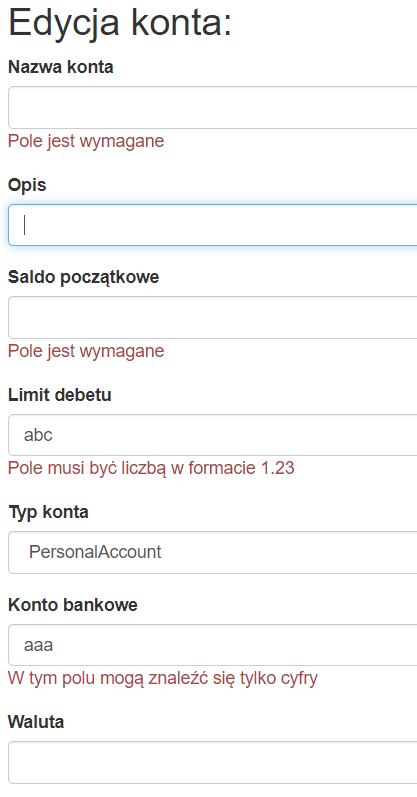
\includegraphics[width=.5\linewidth]{rys05/validation-client-1.PNG}}
	\caption{Struktura fizyczna repozytorium}
	\label{fig:client-test-1}
\end{figure}

\section{Testy API}
\label{sec:test-api}

